
%%%%%%%%%%%%%%%%%%%%%%% file typeinst.tex %%%%%%%%%%%%%%%%%%%%%%%%%
%
% This is the LaTeX source for the instructions to authors using
% the LaTeX document class 'llncs.cls' for contributions to
% the Lecture Notes in Computer Sciences series.
% http://www.springer.com/lncs       Springer Heidelberg 2006/05/04
%
% It may be used as a template for your own input - copy it
% to a new file with a new name and use it as the basis
% for your article.
%
% NB: the document class 'llncs' has its own and detailed documentation, see
% ftp://ftp.springer.de/data/pubftp/pub/tex/latex/llncs/latex2e/llncsdoc.pdf
%
%%%%%%%%%%%%%%%%%%%%%%%%%%%%%%%%%%%%%%%%%%%%%%%%%%%%%%%%%%%%%%%%%%%


\documentclass[runningheads,a4paper]{llncs}

\usepackage{amssymb}
\setcounter{tocdepth}{3}
\usepackage{graphicx}
\graphicspath{ {../} }

\usepackage{url}
\urldef{\mailsa}\path|{thanh.do-chi, quan.dinh-huu-hai, minh.nguyen-binh}@gmail.com|    
\newcommand{\keywords}[1]{\par\addvspace\baselineskip
\noindent\keywordname\enspace\ignorespaces#1}

\usepackage{float}
\usepackage{pdfpages}

\begin{document}

\mainmatter  % start of an individual contribution

% first the title is needed
\title{Cross-platform system to integrate IoT platforms for cross domain applications}

% a short form should be given in case it is too long for the running head
\titlerunning{Cross Platform}

% the name(s) of the author(s) follow(s) next
%
% NB: Chinese authors should write their first names(s) in front of
% their surnames. This ensures that the names appear correctly in
% the running heads and the author index.
%
\author{Thanh Do Chi, Quan Dinh Huu Hai \and Minh Nguyen Binh}
%
\authorrunning{Cross IoT platform}
% (feature abused for this document to repeat the title also on left hand pages)

% the affiliations are given next; don't give your e-mail address
% unless you accept that it will be published
\institute{Ha Noi University of Science and Technology, Viet Nam
\mailsa\\
\url{http://www.soict.hust.edu.vn}}

%
% NB: a more complex sample for affiliations and the mapping to the
% corresponding authors can be found in the file "llncs.dem"
% (search for the string "\mainmatter" where a contribution starts).
% "llncs.dem" accompanies the document class "llncs.cls".
%

\toctitle{Cross IoT Platform}
\tocauthor{Authors' Instructions}
\maketitle


\begin{abstract}
The Internet of Things (IoT) is evolving very quickly. In this IoT world, there are massive of sensors and devices. To management these sensors and devices efficiently, we need IoT platforms, each often suit to a given scenario and use different kind of communication, device control protocols. Because IoT platforms are heterogeneous, which ones usually cannot communicate to each other, the problem of interoperability these IoT platforms is one of the most important and challenging part of IoT. In this paper, we propose a cross-platform layer, which allow integrate new IoT platforms easily, enable interoperability between platforms and also provide APIs for developers create innovative and cross-domain applications.


%\keywords{Internet of Things; cross-platform; interoperability; intergration; cross-domain %applications}


\end{abstract}

\newpage

\section{Introduction}


\hspace*{0.5cm} The Internet of Thing (IoT) is an increasingly hot topic in the tech world. It is part of the theme of digitization. Different types of technology are combining to create digital ecosystems that have potential to drastically improve business processes. There are few interesting statistic on IoT, provided by CMO.com \cite{CMO.com}.

\begin{itemize}
\item In 2008, there were already more \"things\" connected to the Internet than people. By 
2020, the amount of internet-connected things will reach 50 billion, with \$19 trillion in profits and cost savings coming from IoT over the next decade.
\item A whopping 94\% of all businesses have seen a return on their IoT investments.
\item GE estimates that convergence of machines, data, and analytics will become a \$200 billion global industry over the next three years.
\end{itemize}


That interesting IoT industry attract companies to build IoT platforms to manage their own devices and sale to customers. Therefore, there are heterogeneous IoT platforms. Those platforms usually domain-specific, use different of communication technology, represent the devices in different ways, ... According to German IoT market research firm IoT Analytics, the number of IoT platforms on the market has surged 25 percent in just 12 months and now stands at 450 (July 2017) \cite{numberofplatform}.But large number of IoT platforms make it difficult to reuse IoT resources, data between related systems, make it harder to build a IoT ecosystem. An example, a temperature sensor in the house may be managed and seen differently by difference platforms, so it's make redundance of data, hard to control in cross-domain applications. 

\hspace{0.5cm} As the need of building cross-domain applications increasingly, it's raising the need of integrate IoT platforms to a unified cross-platform layer for saving resources, easier to devolope cross-domain applications. To address above mentioned limitations, in this paper, we propose a unified model and an experiment setup result.

This rest of this paper is structured as follows: In section 2, we consider some of the related work about integration of IoT platform. Section 3 introduces out cross-platform model including the architecture of the model, the ontology to presents the sematic of components and the resource graph of a testbed. Section 4 provides result of out experience. Finnaly, we summary the experience and the future work in section 5.

\newpage

\section{Related Work}


Integration is not a new problem in IoT world, there are many research about this area. We will devide them into two aspect of the problem. The first one is architecture of the system, how they build the system, which components do the system have. The second ones see the integration in aspect of ontology, sematic meaning. In each aspect, a lot of studies were introduced to find the unified model for IoT world.\\

On architecture aspect, the Internet of Things Architecture project (IoT-A) \cite{IoT-A} is proposing an architecture reference model for IoT interoperability together with components of future IoT to enable search, discovery and interact as one coherent network.  \\

The IETF \cite{IETF-1}, \cite{IETF-2} community has been involved in foundational IoT technologies such as IPv6 and the Constrained Application Protocol (CoAP), focusing on getting constrained devices and sensor networks connected to the Internet. Similarly, the IEEE \cite{IEEE} has several protocol standards that form the foundation of the IoT and provid connectivity between things and the Internet. \\

HYPERCAT use the concept hub equivalent with IoT platform. It's proposed a four stage path toward interoperability between IoT hubs: 1. \textbf{IoT Core.} Hubs expose things and associated metadata using the web architecture and RESTful web services - a web of things; 2.   \textbf{IoT Model.} Agreement on basic approaches and models requiring a common understanding of what things and  associated data a hub should contain. Achieving this stage will
facilitate the development of adapters and other integration tools for hub interoperability; 3.\textbf{IoT Hub.} Agreement on certain implementation issues such as concrete representations, URLs and schema for describing and querying catalogs and data from hubs. This will include support for security mechanisms so that hubs can control
access to things and offer some guarantees over who is providing things and their data and who is able to access and use these resources. 4.\textbf{IoT Profiles.} Agreement on the semantics of things and their associated data exposed on a hub. For example: a temperature sensor in one hub provides the same quality and value of temperature as one in another hub. Essentially the taxonomy of things and the ontological models that hubs support will need to be defined. By reaching agreement at this level, deep integration of application is possible, allowing hubs and things to link to and communicate directly with each other. \\

Although these work are making IoT interoperability closer, but some has it's limitation. Such as IETF and IEEE primarily focus on connect things to the internet. IoT-A project is a ambitious standardization effort but it's too big, maybe attempting to lock down aspect of IoT ecosystem while it is still evolve rapidly. Developers and vendors however, may favour less complex approaches that address requirements as they emerge. HYPERCAT according our opinion, follow the best practices and our work are independent but quite homologous with it. But HYPERCAT has some problems : platforms/hubs in the project are closed platform, it's make developer harder to reimplement to paper. Our proposal are implemented on three open source platforms are Home Assitant \cite{home-assistant}, OpenHAB \cite{openhab}, ThingsBoard \cite{thingsboard} which are the most popular opensource IoT platforms, large commudity and well documented. \\



Ontology ...\\
Ontology ...\\
Ontology ...\\\\
Ontology ...\\
Ontology ...\\
Ontology ...\\\\
Ontology ...\\\\
Ontology ...\\


\newpage

\section{Cross-platform model}

\subsection{Deployment Architecture}

\begin{figure}[h]
\centering
\includegraphics[scale=0.4]{services} 
\caption{Deploy architecture}
\end{figure}


The deployment architecture has three layers, including:

\begin{itemize}

\item \texttt{End-Devices}. This layer contains every IoT Things: sensors, intelligence devices, actuators.

\item \texttt{Fog} IoT devices are sending data high frequently, so it is usually that data will not send directly to cloud but to fog layer cause of fog layer nearer to the IoT devices will help reduce the cost of bandwith, storage and reduce the delay between cloud and devices. IoT platforms installed on the Fog layer to manage the devices. To build a system integrate many platforms, we write a driver for each platform to tranforms the data models, generated and APIs which platforms provided into unified data and API. For further purpose, some other modules also implemented such as Filter (to filter the data), Forwarder (to forward the data from Fog to Cloud), ... 

\item \texttt{Cloud} Fog layer often has low computational capacity, so we need to build main 
processing modules on the Cloud. Cloud layer use data received from \texttt{Fog} to manage information and data from platforms, devices in platforms. Once a platform join the system, it have to send meta data about it to Registry module. Registry will check if it had information of this platform, if not, Registry will provides unique ID for all devices in the platform. All devices data and platform information stored in a database. Also, Single Unified Interface converts APIs of different platforms into unified API.

\end{itemize}

System's modules had built following microservices architecture so it's flexible to remove, add and change a service. 


\subsection{Ontology}

\begin{figure}[H]
\centering
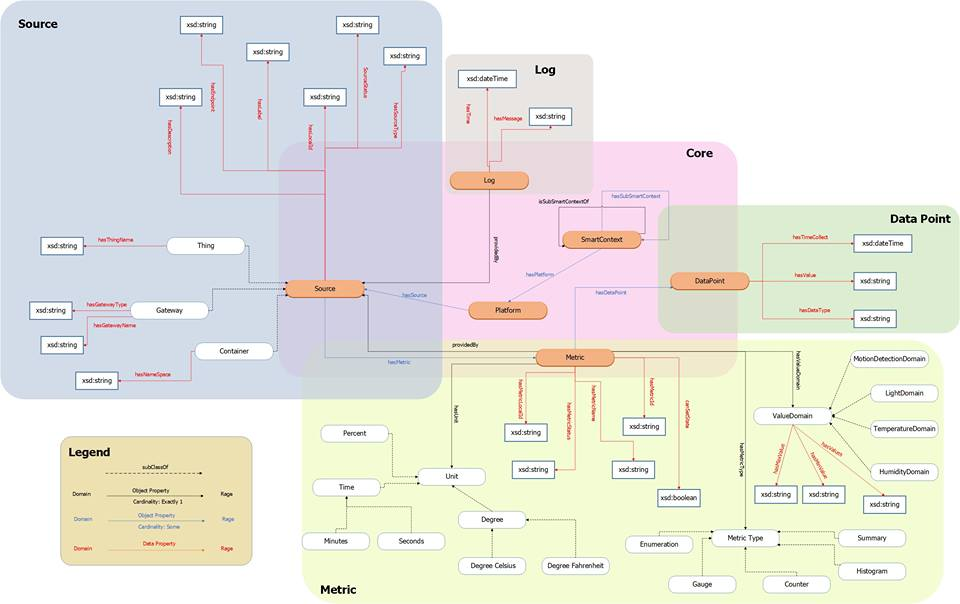
\includegraphics[scale=0.4]{ontology}
\caption{Cross-platform ontology.}
\end{figure}

\begin{itemize}
\item \textbf{Smart Context} is the root of the graph, which is a testbed implemeted of the cross-platform system. It can be a smart home, smart building, smart city, ... One \texttt{Smart Context} maybe is a sub smart context of another smartcontext; and a smart context maybe has one or many sub smart context.

\item \textbf{Platform} is \texttt{a multi-layer technology that enables straightforward provisioning, management, and automation of connected devices within the Internet of Things universe. It basically connects your hardware, however diverse, to the cloud by using flexible connectivity options, enterprise-grade security mechanisms, and broad data processing powers} \cite{platform}. 

\item \textbf{Source} is physical or vitrual devices. Source generate data about evironment or anything it monitor. A \textbf{Source} might be a \textbf{Thing}, a \textbf{Gateway} or a \textbf{Processing Unit}.
 
\item \textbf{Thing} is a device which is a set of sensors. 

\item \textbf{Gateway} is a physical device or software program that servers as the connection point between the cloud and controllers, sensors and intelligence devices.

\item \textbf{Processing Unit} is a virtual device to monitor devices's resource in the IOT system like CPU, memory, storage, ... 

\item \textbf{Log} is the data generated from \textbf{Sources}. Log file can use to extract historical information, monitor devices's status, use in alert services and rule engine, ...

\item \textbf{Metric} is used to express diverse metric types of the collected data such as \textbf{Enumeration}, \textbf{Gauge}, \textbf{Counter}, \textbf{Histogram}, \textbf{Summary}. Each Metric has it's own \textbf{Unit} which might be \textbf{Percent}, \textbf{Time}, \textbf{Degree}. Metric connected to Source mean that each Source correspond to a Metric.

\item \textbf{Data Point} is generated when a \textbf{Source} active. Based on \texttt{Metric} information of a \textbf{Source}, data generate will have suitable DataType and DataValue.
\end{itemize}

\subsection{Resource Graph}
Once we have the cross-platform system, we will need to integrate testbeds with it. One of the first step we need to care about is registration all its devices and services. The figure below show the resource graph from SmartBuilding testbed. \\

\begin{figure}[H]
\centering
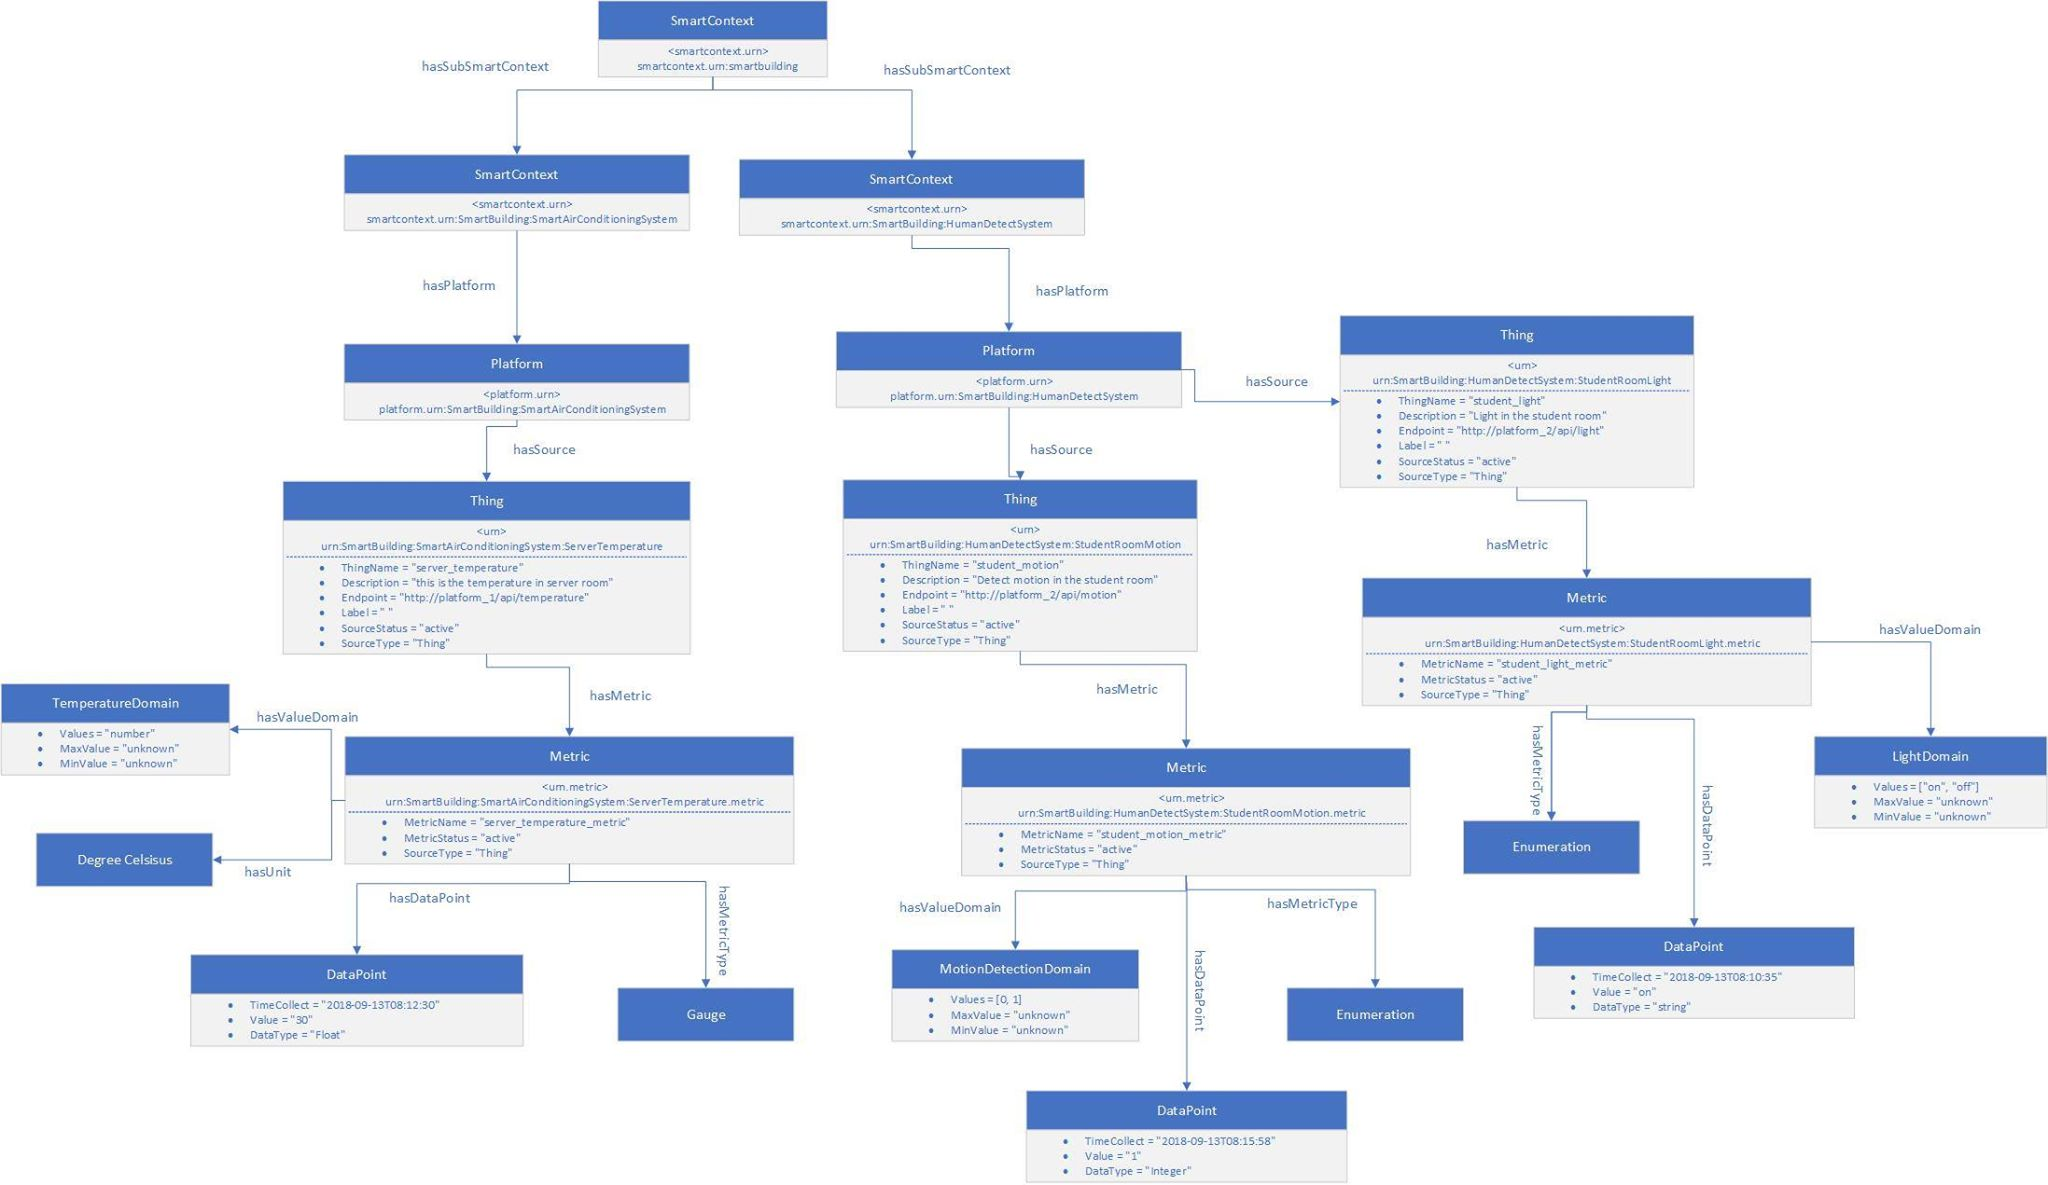
\includegraphics[scale=0.2]{resource_graph} 
\caption{Resource graph}
\end{figure} 

Anotation for the resource graph: \\

\begin{itemize}
\item smartcontext.um:SmartBuilding is a \texttt{Smart Context} \\
\hspace*{0.5cm} hasSubSmartContext smartcontext.um:SmartBuilding:SmartAirconditionSystem \\
\item smartcontext.um:SmartBuilding:SmartAirconditionSystem is a \texttt{Smart Context} \\ 
\hspace*{0.5cm} hasPlatform platform.um:SmartBuilding:SmartAirconditionSystem \\
\item platform.um:SmartBuilding:SmartAirconditionSystem is a \texttt{Platform} \\
\hspace*{0.5cm} hasSource urn:SmartBuilding:SmartAirconditionSystem:ServerTemperature	\\
\item urn:SmartBuilding:SmartAirconditionSystem:ServerTemperature is a \texttt{Thing} \\
\hspace*{0.5cm} ThingName "server\_temperature" \\ 
\hspace*{0.5cm} Description "this is the temperature in server room" \\
\hspace*{0.5cm} Endpoint "http://platform\_1/api/temperature" \\ 
\hspace*{0.5cm} Label "" \\
\hspace*{0.5cm} SourceStatus "active" \\
\hspace*{0.5cm} SourceType "Thing" \\
\hspace*{0.5cm} hasMetric urn:SmartBuilding:SmartAirconditionSystem:ServerTemperature.metric \\
\item urn:SmartBuilding:SmartAirconditionSystem:ServerTemperature.metric is a \texttt{Metric}\\
\hspace*{0.5cm} MetricName "server\_temperature\_metric"\\
\hspace*{0.5cm} MetricStatus "active"\\
\hspace*{0.5cm} SourceType "Thing"\\
\hspace*{0.5cm} hasValueDomain TemperatureDomain\\
\hspace*{0.5cm} hasUnit Degree Celsisus\\
\hspace*{0.5cm} hasDataPoint DataPoint\\
\hspace*{0.5cm} hasMetricType Gauge\\
\end{itemize}

%\newpage
\section{Deploy IoT Platforms}
\subsection{Target}
\begin{itemize}
\item Deploy IoT Platforms and related devices
\item Testing with devices (collect data, turn on/off led, ...)\\
\end{itemize}

\subsection{Implement}

In this section, we will deploy 3 platforms: Home Assistant, OpenHAB and ThingsBoard. Each IoT Platform is deployed on different side, and combine:\\

\begin{itemize}
\item 1 temperature sensor\\
\item 1 humidity sensor\\
\item 1 photo sensor\\
\item 1 motion sensor\\
\item 3 LEDs\\
\end{itemize}

Deployed model on each IoT platform as figure:\\
\begin{figure}[H]
\centering
\includegraphics[width=1\textwidth, height=0.8\textheight]{deployIoTPlatform} 
\caption{Deploy model}
\end{figure} 

To collect data, we connected sensors and LEDs to a Arduino. This Arduino responsibility for collect data and forward data to ESP8266. We have to use ESP8266 because Arduino is not able  to connect to the network. ESP8266 forward data to one of three above IoT platforms deployed on Raspery Pi 3 in the same LAN.\\

\subsection{Result and Conclusion}
After deployment, the result we have three IoT platforms with user interfaces below:\\

\begin{figure}[H]
\centering
\includegraphics[scale=0.3]{home-assistant} 
\caption{User Interface of Home Assistant}
\end{figure} 



\begin{figure}[H]
\centering
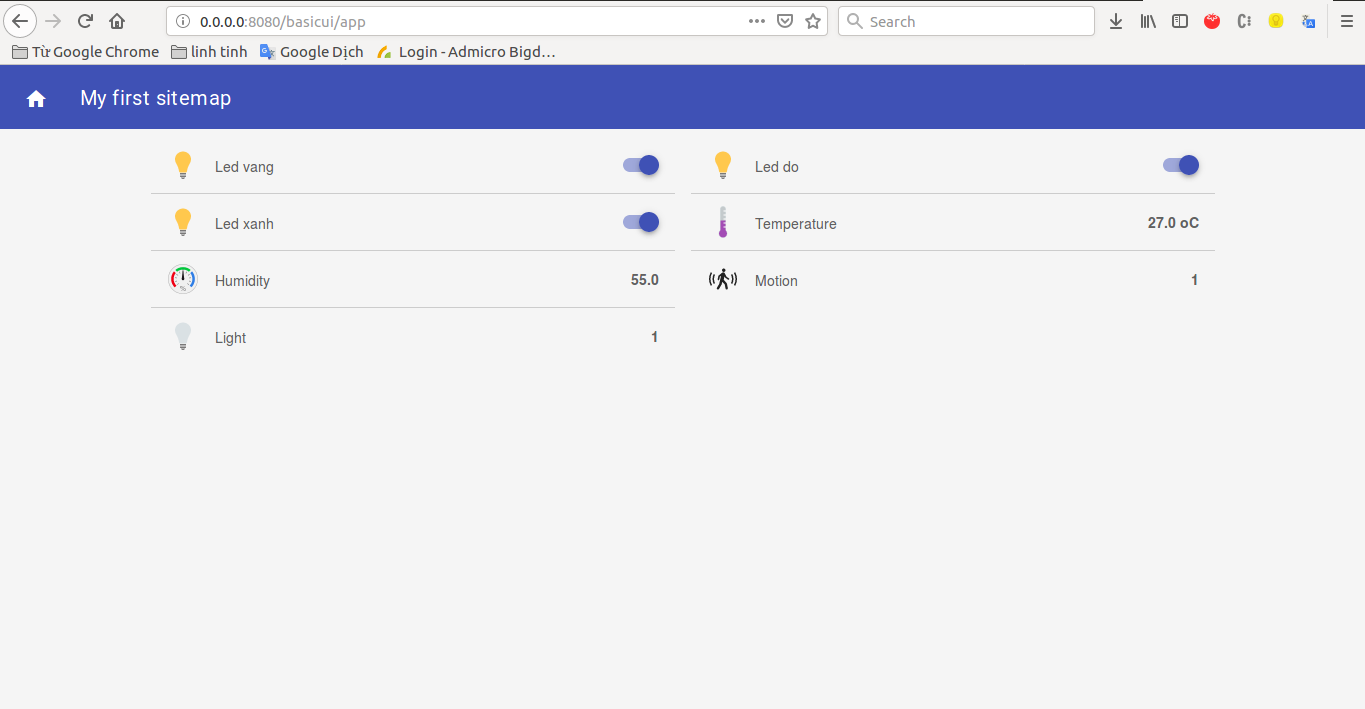
\includegraphics[scale=0.3]{openhab} 
\caption{User Interface of OpenHAB}
\end{figure} 


\begin{figure}[H]
\centering
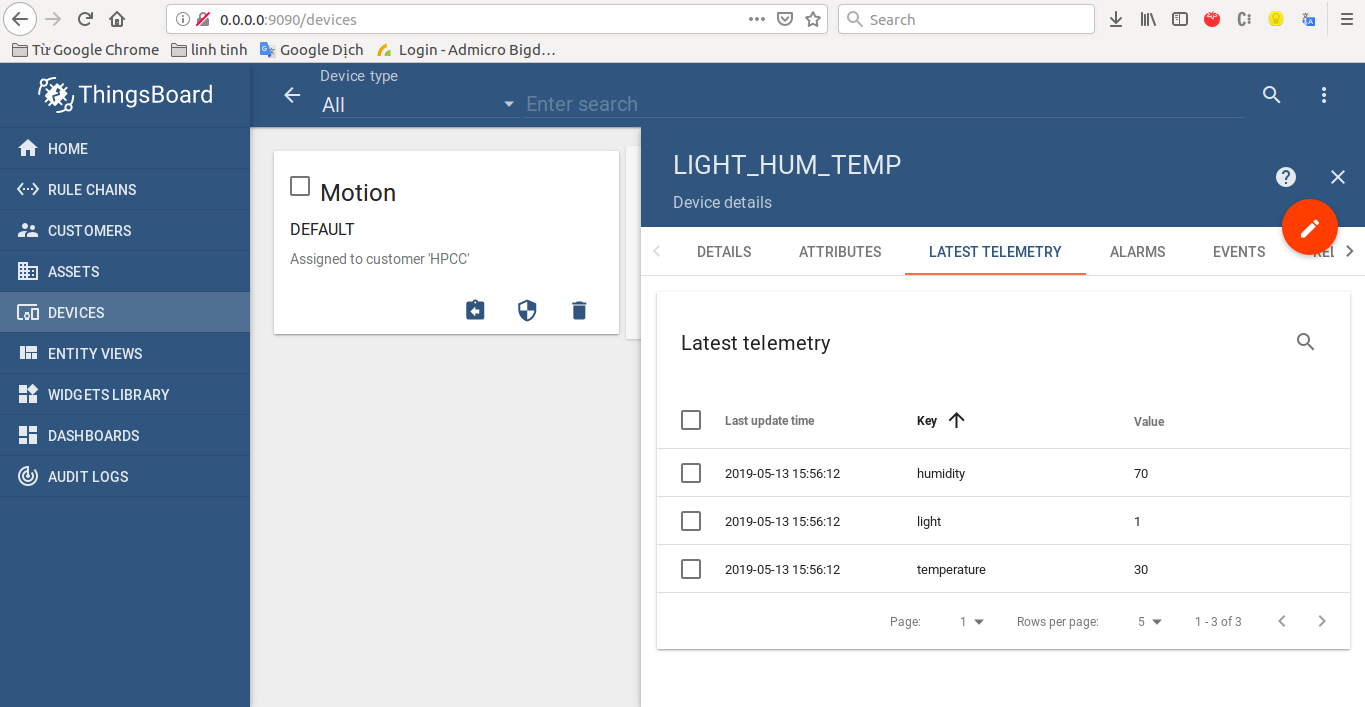
\includegraphics[scale=0.3]{thingsboard} 
\caption{User interface of Thingsboard}
\end{figure} 


\section{Implement a Alert application with data collected from 3 IoT platforms}
\subsection{Target}
\begin{itemize}
\item Demonstrate that our cross-platform system can collect data from many IoT platforms.
\item Demonstrate our released API can provide for developers to use them easily depend on demand.
\end{itemize}


\subsection{Implementation}
We will build a simple application. The model of this application as follow

\begin{figure}[H]
\centering
\includegraphics[scale=0.8]{monitor} 
\caption{Application model}
\end{figure} 

The application monitor data collected from three platforms: Home Assistant, OpenHAB and ThingsBoard.

\begin{itemize}
\item Home Assistant: Data from temperature sensor
\item OpenHAB: Data from humidity sensor
\item ThingsBoard: Data from motion sensor
\end{itemize}


\begin{figure}[H]
\centering
\includegraphics[scale=0.3]{MonitoringApplication} 
\caption{Communication Diagram of monitor application}
\end{figure} 


Application monitor the data and generate a alert on the interface when all following condition are satisfied:

\begin{itemize}
\item Temperature greater than 35 Cencius degree
\item Humidity less than 50 percent
\item There is a motion on the monitering region
\end{itemize}


\subsection{Result}

\begin{figure}[H]
\centering
\includegraphics[scale=0.3]{UI_monitor_application_1} 
\caption{Monitoring Application interface}
\end{figure} 


\begin{figure}[H]
\centering
\includegraphics[scale=0.4]{UI_monitor_application_2} 
\caption{Monitoring Application interface with alert}
\end{figure} 


\section{Experiment}

\subsection{Target}
\begin{itemize}
\item Measure some operation runtime of the system to see some characteristic and conclusion  
\end{itemize}

\subsection{Implementation}

In this section, we build a simple program to collect continous data and tuning devices status. Implementation process is describe in the below diagram.

\begin{figure}[H]
\centering
\includegraphics[scale=0.6]{script_test} 
\caption{Implementation process}
\end{figure} 


\begin{figure}[H]
\centering
\includegraphics[scale=0.5]{response_IoTPlatform} 
\caption{Communication Diagram Collecting data from IoT platform}
\end{figure} 


\begin{figure}[H]
\centering
\includegraphics[width=1.1\textwidth, height=0.6\textheight]{update_data} 
\caption{Communication Diagram Updating data into our system}
\end{figure} 


\begin{figure}[H]
\centering
\includegraphics[width=1.1\textwidth, height=0.6\textheight]{get_states} 
\caption{Communication Diagram Getting data from a device}
\end{figure} 


With above process, we tuning config variables of the system, make test cases and measure carefully to get the best configuration on different cases. We consider some cases:

\begin{itemize}
\item Number of sensors: 25 sensors, 50 sensors, 100 sensors
\item Data frequency: 1 second, 1.5 second, 2 second (per data point)
\end{itemize}   


\subsection{Result and Conclusion}
\subsubsection{Runtime of basic APIs}

We measure runtime of three API that are  most used:

\begin{itemize}
\item API to get list all IoT platforms in the system
\item API to get list all devices on a specific platform
\item API to get a specific device on the system
\end{itemize}




\begin{figure}[H]
\centering
\includegraphics[page=1, width=1.2\textwidth, height=1.4\textheight]{bang_1} 
\caption{Average result when change number of device}
\end{figure} 

\begin{figure}[H]
\centering
\includegraphics[page=2, width=1.2\textwidth, height=1.4\textheight]{bang_1} 
\caption{Average result when change number of device}
\end{figure} 

\begin{figure}[H]
\centering
\includegraphics[page=3, width=1.2\textwidth, height=1.4\textheight]{bang_1} 
\caption{Average result when change number of device}
\end{figure} 




\begin{figure}[H]
\centering
\includegraphics[width=1.1\textwidth, height=0.6\textheight]{time-api} 
\caption{Average result when change number of device}
\end{figure} 

We can conclude: 

\begin{itemize}
\item Time to get list all IoT platforms is unchange when changing number of device.
\item Time to get list all devices of a specific platform will increase when number of devices increase and vice versa. This is understanable because of:
\begin{itemize}
\item Work with database: Increase number of device will increase respond time and query time in database.
\item Tranfer time: Larger amount of data will cost more time to tranfer
\end{itemize}

\item Even time to get list all devices increase when number of device increase but with 100 device, the API respond time is less than 1 second. We think this respond time is acceptable.
\item Time to get a specific device on the system is unchange when changing number of device
\end{itemize}


\subsubsection{Runtime of some tasks}

In this experiment, we test with different number of device, data frequency to measure runtime of some tasks:

\begin{itemize}
\item Respond time of IoT platforms when system query data
\item Update time when update new data into system
\item API runtime to get new data of a device
\item API runtime to set new state for a device
\end{itemize}



\begin{figure}[H]
\centering
\includegraphics[page=1, width=1.2\textwidth, height=1.4\textheight]{bang_2} 
\caption{Average result when change number of device}
\end{figure} 

\begin{figure}[H]
\centering
\includegraphics[page=2, width=1.2\textwidth, height=1.4\textheight]{bang_2} 
\caption{Average result when change number of device}
\end{figure} 

\begin{figure}[H]
\centering
\includegraphics[page=3, width=1.2\textwidth, height=1.4\textheight]{bang_2} 
\caption{Average result when change number of device}
\end{figure} 




\begin{figure}
\centering
\includegraphics[width=1.1\textwidth, height=0.6\textheight]{time_service_source} 
\caption{Average result when change number of device}
\end{figure} 


We have conclusion:

\begin{itemize}
\item Respond time of IoT platforms change when change number of device. This is understandable because managing large amount of device need more time to process.
\item Update time when update new data into system increase linearly with number of device. 	The reason is more data also mean need more time to tranfer and more read/write operation on database.
\item API runtime to get new data of a device is stable when number of device changing. This mean the system is stable with end user when the system get larger
\item API runtime to set new state for a device increase when increase the number of device. It's not mean the system process inefficiently but because of above reason: IoT platforms respond and process slowly when number of device get large.
\end{itemize}



\begin{figure}[H]
\centering
\includegraphics[page=1, width=1.2\textwidth, height=1.4\textheight]{bang_3} 
\caption{Average result when change number of device}
\end{figure} 

\begin{figure}[H]
\centering
\includegraphics[page=2, width=1.2\textwidth, height=1.4\textheight]{bang_3} 
\caption{Average result when change number of device}
\end{figure} 

\begin{figure}[H]
\centering
\includegraphics[page=3, width=1.2\textwidth, height=1.4\textheight]{bang_3} 
\caption{Average result when change number of device}
\end{figure} 




\begin{figure}
\centering
\includegraphics[width=1.1\textwidth, height=0.6\textheight]{time_service_time} 
\caption{Average result when change frequency send data}
\end{figure} 


We have conclusion:

\begin{itemize}
\item Respond time of IoT platforms when system query data is not changing too much if change frequent sending data and the number of device unchange.
\item Update time when update new data into system is not changing too much if change frequent sending data and the number of device unchange.
\item  API runtime to get new data of a device is stable even increase number of device and frequent sending data.
\item API runtime to set new state for a device will increase if increase frequent sending data. The reason is platforms need to update a lot of data when increase frequent sending data and respond slowly.
\end{itemize}


\newpage
\section{Conclusion}

With the results introduced above, we haved demonstrated that:

\begin{itemize}
\item Our Cross-platform can collect, monitoring data from different IoT platforms. We just present a simple monitoring application here but in the large scale, we can scale up the system and do complex tasks on different IoT platforms, which is impossible if IoT platforms work independently.
\item Our APIs provide for developer to build applications on many domain and cross-domain easily.
\end{itemize}

\section{The References Section}\label{references}

\begin{thebibliography}{4}

\bibitem{platform} https://www.kaaproject.org/what-is-iot/ \\

\bibitem{CMO.com} https://www.cmo.com/features/articles/2015/4/13/mind-blowing-stats-internet-of-things-iot.html\#gs.NxjVM9k1 \\

\bibitem{numberofplatform} https://iot-analytics.com/iot-platforms-company-list-2017-update/

\bibitem{IoT-A} "Internet of Things - Architecture — IOT-A: Internet of ThingsArchitecture."    http://www.iot-a.eu/public.[Accessed: 28-May-2013]

\bibitem{IETF-1} "IEEE-SA - Internet of Things Related Standards." http://standards.ieee.org/innovate/iot/stds.html.         

\bibitem{IETF-2} A. P. Castellani, M. Gheda, N. Bui, M. Rossi, and M. Zorzi, “WebServices for the Internet of Things through CoAP and EXI,” in 2011IEEE International Conference on Communications Workshops (ICC),2011, pp. 1–6

\bibitem{IEEE} “IEEE-SA - Internet of Things Related Standards.” [Online]. http://standards.ieee.org/innovate/iot/stds.

\bibitem{home-assistant} https://www.home-assistant.io/

\bibitem{openhab} https://www.openhab.org/

\bibitem{thingsboard} https://thingsboard.io/


\end{thebibliography}

\end{document}
